\documentclass[11pt]{beamer}

% Hỗ trợ tiếng Việt
\usepackage[utf8]{vietnam}
\usepackage{graphicx}
\usepackage{tikz} 
\usetikzlibrary{positioning, arrows.meta}

% Giao diện slide
\usetheme{Madrid}
\usecolortheme{default}

% ==========================================
% ĐỔI MÀU & CHÂN TRANG
% ==========================================
\definecolor{DarkTeal}{RGB}{0, 80, 80}
\definecolor{OrangeAccent}{RGB}{255, 150, 0}
\definecolor{myblue}{RGB}{0, 114, 178} % Màu dùng trong TikZ của bạn
\definecolor{myorange}{RGB}{213, 94, 0} % Màu dùng trong TikZ của bạn

\setbeamercolor{structure}{fg=DarkTeal}
\setbeamercolor{palette primary}{bg=DarkTeal, fg=white}
\setbeamercolor{palette secondary}{bg=OrangeAccent, fg=white}
\setbeamercolor{palette tertiary}{bg=DarkTeal!90, fg=white}
\setbeamercolor{frametitle}{bg=DarkTeal, fg=white}

% Cài đặt màu cho các hộp (box) của bạn
\setbeamercolor{block title}{bg=DarkTeal, fg=white}
\setbeamercolor{block body}{bg=DarkTeal!10, fg=black}
\setbeamercolor{block title alerted}{bg=OrangeAccent, fg=white}
\setbeamercolor{block body alerted}{bg=OrangeAccent!10, fg=black}

\setbeamertemplate{navigation symbols}{} % Ẩn thanh điều hướng

% Tùy chỉnh chân trang
\setbeamertemplate{footline}{
  \leavevmode%
  \hbox{%
  \begin{beamercolorbox}[wd=.333333\paperwidth,ht=2.25ex,dp=1ex,center]{palette tertiary}%
    \usebeamerfont{author in head/foot}\insertshortauthor
  \end{beamercolorbox}%
  \begin{beamercolorbox}[wd=.333333\paperwidth,ht=2.25ex,dp=1ex,center]{palette secondary}%
    \usebeamerfont{title in head/foot}LÝ THUYẾT ĐỒ THỊ
  \end{beamercolorbox}%
  \begin{beamercolorbox}[wd=.333333\paperwidth,ht=2.25ex,dp=1ex,right]{palette primary}%
    Học kỳ II - 2026 \hspace*{2em}
    \insertframenumber{} / \inserttotalframenumber \hspace*{2ex} 
  \end{beamercolorbox}}%
  \vskip0pt%
}

% ==========================================
% ĐỊNH NGHĨA MÔI TRƯỜNG THEO CODE CỦA BẠN
% ==========================================
\newenvironment{mainbox}[1]{\begin{block}{#1}}{\end{block}}
\newenvironment{highlightbox}[1]{\begin{alertblock}{#1}}{\end{alertblock}}

% Thông tin cơ bản
\author[Tung Tung Tung Sahur]{Tung Tung Tung Sahur}

\begin{document}

% ==========================================
% PHẦN 4: BÀI TOÁN HAY (TỪ ẢNH 2 & 3)
% ==========================================
\section{Bài toán hay}

\begin{frame}{ PHẦN 4: Một số bài toán hay }
    \begin{center}
    \end{center}
    \vspace{0.3cm}
    \begin{columns}[T]
        \begin{column}{0.48\textwidth}
            \begin{mainbox}{1. 7 cây cầu Königsberg}
                Bài toán kinh điển dẫn đến sự ra đời của Lý thuyết đồ thị.
            \end{mainbox}
            \vspace{0.2cm}
            \begin{mainbox}{2. Tô màu bản đồ}
                Định lý 4 màu và các ứng dụng trong thực tế.
            \end{mainbox}
        \end{column}
        \begin{column}{0.48\textwidth}
            \begin{mainbox}{3. Đường đi ngắn nhất}
                Tối ưu hóa hành trình từ A đến B trong thực tế.
            \end{mainbox}
            \vspace{0.2cm}
            \begin{mainbox}{4. Mạng xã hội}
                Phân tích ai là người "trung tâm" của đám đông.
            \end{mainbox}
        \end{column}
    \end{columns}
\end{frame}

% --- CHI TIẾT BÀI TOÁN 1 ---
\begin{frame}{1. Bài toán 7 cây cầu (Seven Bridges)}
    \begin{columns}[T]
        \begin{column}{0.6\textwidth}
            \begin{mainbox}{Lịch sử \& Thách thức}
                Thành phố Königsberg có 7 cây cầu nối các vùng đất. Câu hỏi: \textbf{Có thể đi qua mỗi cầu đúng 1 lần rồi quay về?}
            \end{mainbox}
            \vspace{0.3cm}
            \begin{highlightbox}{Kết luận của Euler}
                $\rightarrow$ \textbf{KHÔNG THỂ!} 
                Vì số lượng cầu (cạnh) nối vào mỗi vùng đất (đỉnh) phải là số chẵn.
            \end{highlightbox}
        \end{column}
        \begin{column}{0.35\textwidth}
            \begin{center}
                \textit{(Hình minh họa)} \\
                \begin{tikzpicture}
                    \node[draw, fill=gray!20, minimum size=1cm] (island) {Đảo};
                    \foreach \a in {45, 90, 135, 225, 270, 315, 0}
                        \draw (island) -- (\a:1.5cm);
                \end{tikzpicture}
            \end{center}
        \end{column}
    \end{columns}
\end{frame}

% --- CHI TIẾT BÀI TOÁN 2 ---
\begin{frame}{2. Bài toán tô màu bản đồ}
    \begin{columns}[T]
        \begin{column}{0.5\textwidth}
            \begin{mainbox}{Định lý 4 màu}
                Mọi bản đồ trên mặt phẳng đều có thể tô bằng \textbf{tối đa 4 màu} mà không có hai vùng láng giềng nào trùng màu nhau.
            \end{mainbox}
        \end{column}
        \begin{column}{0.5\textwidth}
            \begin{highlightbox}{Ứng dụng thực tế}
                \begin{itemize}
                    \item Sắp xếp lịch thi cử tránh trùng môn.
                    \item Cấp phát tần số cho các trạm phát sóng điện thoại.
                \end{itemize}
            \end{highlightbox}
        \end{column}
    \end{columns}
\end{frame}

% --- CHI TIẾT BÀI TOÁN 4 ---
\begin{frame}{4. Bài toán mạng xã hội}
    \begin{mainbox}{Ai là người "trung tâm"?}
        Trong một mạng lưới kết nối, việc tìm ra người quan trọng nhất dựa trên:
        \begin{itemize}
            \item \textbf{Degree Centrality:} Ai có nhiều bạn nhất?
            \item \textbf{Betweenness Centrality:} Ai là "cầu nối" duy nhất giữa các nhóm?
        \end{itemize}
    \end{mainbox}
    \vspace{0.3cm}
    \begin{center}
        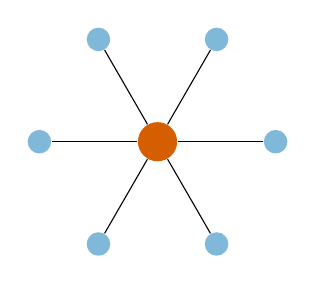
\begin{tikzpicture}
            \node[circle, fill=myorange, inner sep=5pt] (hub) at (0,0) {};
            \foreach \i in {1,...,6} {
                \node[circle, fill=myblue!50, inner sep=3pt] (n\i) at (\i*60:1.5) {};
                \draw (hub) -- (n\i);
            }
        \end{tikzpicture}
    \end{center}
\end{frame}

\end{document}
